\begin{figure}[h]
  \centering
  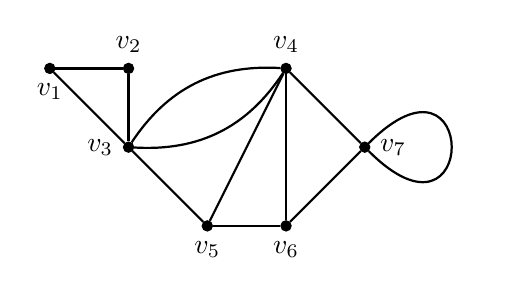
\begin{tikzpicture}
\tikzset{enclosed/.style={draw, circle, inner sep=0pt, minimum size=.13cm, fill=black}}
    \node[enclosed] at (1,2) (v2) [label=above:\(v_2\)] {};
    \node[enclosed] at (3,2) (v4) [label=above:\(v_4\)] {};
    \node[enclosed] at (4,1) (v7) [label=right:\(v_7\)] {};
    \node[enclosed] at (2,0) (v5) [label=below:\(v_5\)] {};
    \node[enclosed] at (3,0) (v6) [label=below:\(v_6\)] {};
    \node[enclosed] at (1,1) (v3) [label=left:\(v_3\)] {};
    \node[enclosed] at (0,2) (v1) [label=below:\(v_1\)] {};
    
    \path[thick] (v1) edge node[midway, above] {} (v2);
    \path[thick] (v4) edge[bend right] node[midway, above] {} (v3);
    \path[thick] (v3) edge node[midway, above] {} (v2);
    \path[thick] (v3) edge[bend right] node[midway, above] {} (v4);
    \path[thick] (v4) edge node {} (v5);
    \path[thick] (v4) edge node {} (v6);
    \path[thick] (v4) edge node {} (v7);
    \path[thick] (v7) edge node {} (v6);
    \path[thick] (v6) edge node {} (v5);
    \path[thick] (v5) edge node {} (v3);
    \path[thick] (v1) edge node {} (v3);
    \path[thick] (v7) edge [out=315,in=45,looseness=50] node[right] {} (v7);


  \end{tikzpicture}
  \caption{Ikke-orienteret pseudograf.}
  \label{fig:ikke-orienteret-pseudo}
\end{figure}


\begin{table}[h]
	\centering
	\begin{tabular}{ |p{3cm}|p{3cm}|}
 		\hline
 		Knuder & Naboknuder\\
 		\hline
 		$v_1$ & $v_2$, $v_3$\\
		$v_2$ & $v_1$, $v_3$ \\
		$v_3$ & $v_1$, $v_2$, $v_4$, $v_5$ \\
		$v_4$ & $v_3$, $v_5$, $v_6$, $v_7$ \\
		$v_5$ & $v_3$, $v_4$, $v_6$ \\
		$v_6$ & $v_4$, $v_5$, $v_7$ \\
		$v_7$ & $v_4$, $v_6$, $v_7$ \\
 		\hline 
	\end{tabular}
	\caption{Naboliste til figur \ref{fig:ikke-orienteret-pseudo}.}
	\label{tab:naboliste-ikke-orienteret}
\end{table}
